\chapter{Analog In with an Arduino}

In this lab, you'll learn how to connect a variable resistor to a microcontroller and read it as an analog input. You'll be able to read changing conditions from the physical world and convert them to changing variables in a program.

For this lab you will need to have the following parts:

Solderless breadboard

\begin{figure}[!htb]
 \centering
 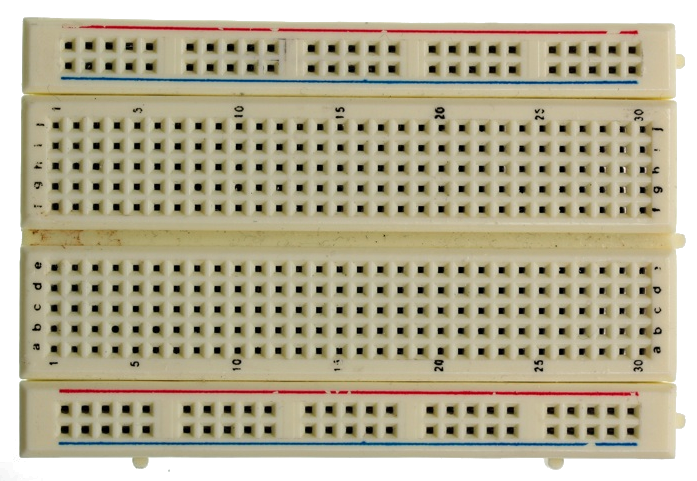
\includegraphics[scale=0.3]{img/analogio/breadboard.png}
 \caption{Solderless breadboard}
 \label{Solderless breadboard}
\end{figure}

22-AWG hookup wire

\begin{figure}[!htb]
 \centering
 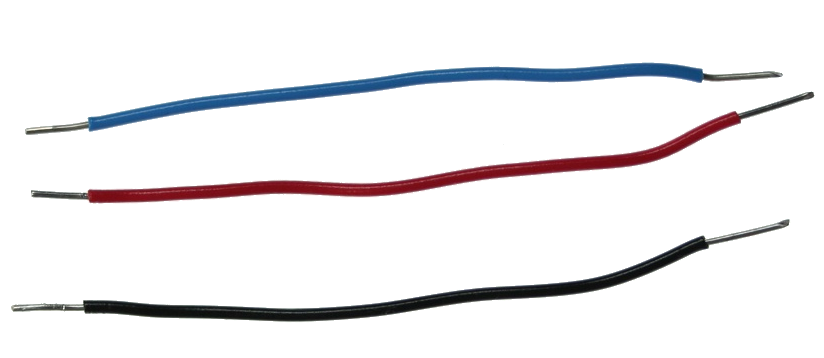
\includegraphics[scale=0.3]{img/analogio/hookup_wire.png}
 \caption{22-AWG hookup wire}
 \label{22-AWG hookup wire}
\end{figure}

Arduino Microcontroller module

\begin{figure}[!htb]
 \centering
 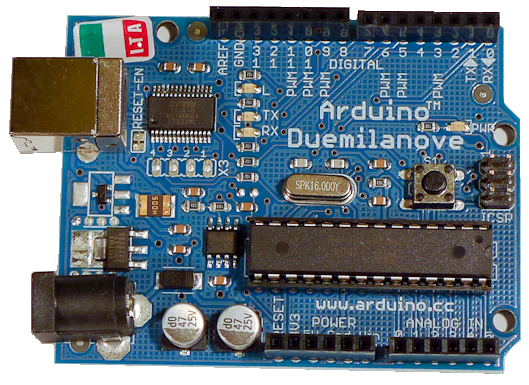
\includegraphics[scale=0.3]{img/analogio/arduino.png}
 \caption{arduino}
 \label{arduino}
\end{figure}

Light Emiting Diodes, LED


\begin{figure}[!htb]
 \centering
 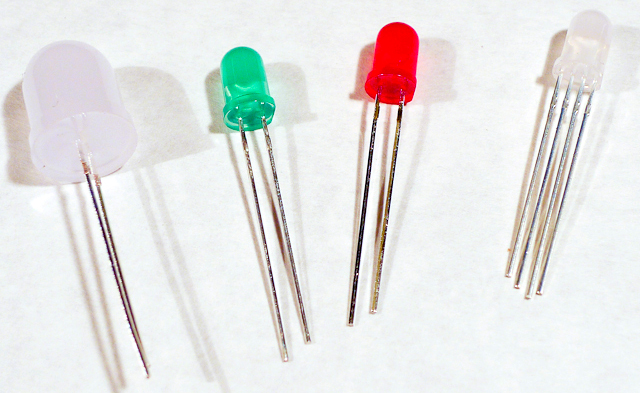
\includegraphics[scale=0.3]{img/analogio/leds.jpg}
 \caption{leds}
 \label{leds}
\end{figure}

220-ohm and 10Kohm resistors


\begin{figure}[!htb]
 \centering
 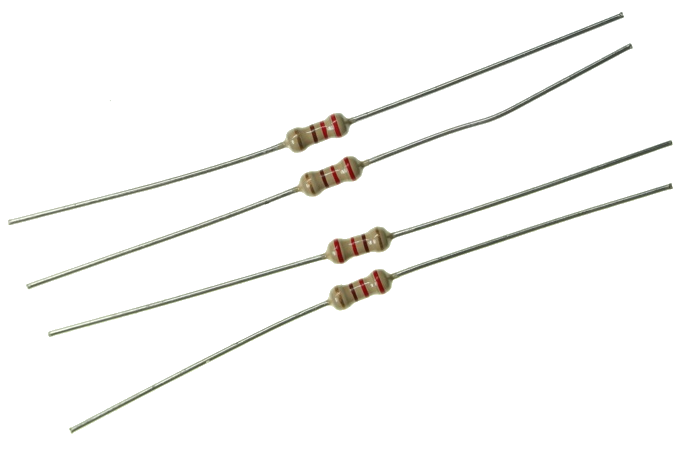
\includegraphics[scale=0.3]{img/analogio/resistors_220.png}
 \caption{resistors 220}
 \label{resistors 220}
\end{figure}

10Kohm potentiometer

\begin{figure}[!htb]
 \centering
 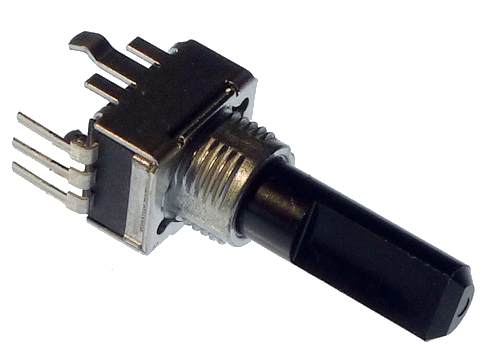
\includegraphics[scale=0.3]{img/analogio/potentiometer.png}
 \caption{potentiometer}
 \label{potentiometer}
\end{figure}

Variable resistors


\begin{figure}[!htb]
 \centering
 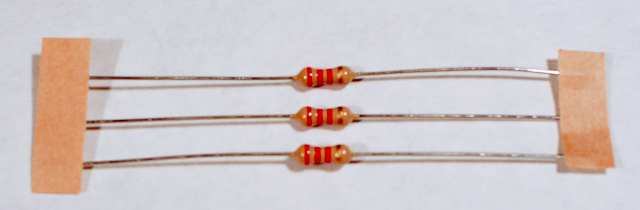
\includegraphics[scale=0.3]{img/analogio/resistors.jpg}
 \caption{resistors}
 \label{resistors}
\end{figure}

Flex sensors (or a different form of variable resistor)

\begin{figure}[!htb]
 \centering
 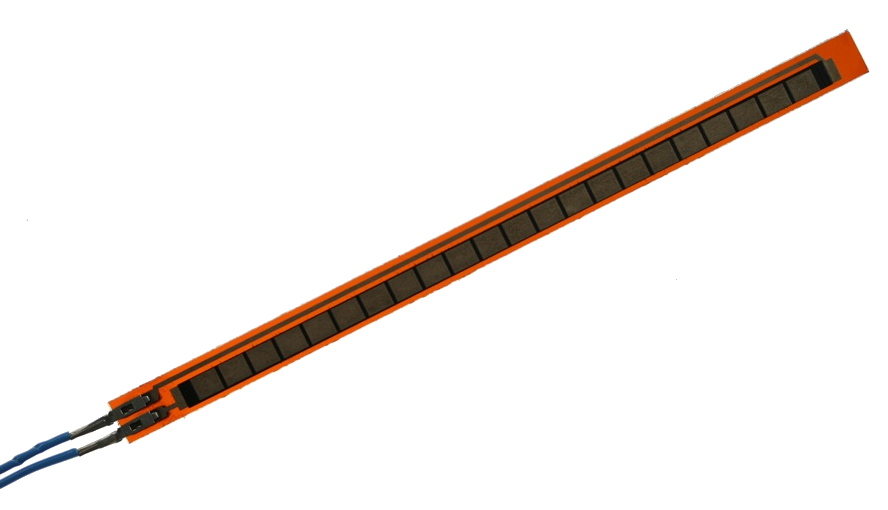
\includegraphics[scale=0.3]{img/analogio/flex_sensors.png}
 \caption{flex sensors}
 \label{flex sensors}
\end{figure}


\section{Prepare the breadboard}

Conect power and ground on the breadboard to power and ground from the microcontroller. On the Arduino module, use the 5V and any of the ground connections:

\begin{figure}[!htb]
 \centering
 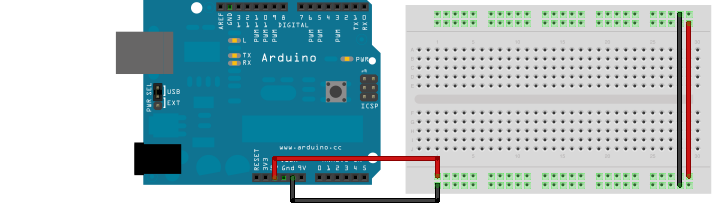
\includegraphics[scale=0.3]{img/analogio/arduino_and_breadboard_bb.png}
 \caption{arduino and breadboard bb}
 \label{arduino and breadboard bb}
\end{figure}

\section{Add a potentiometer and LED}

Connect a potentiometer to analog in pin 0 of the module, and an LED to digital pin 9:

\begin{figure}[!htb]
 \centering
 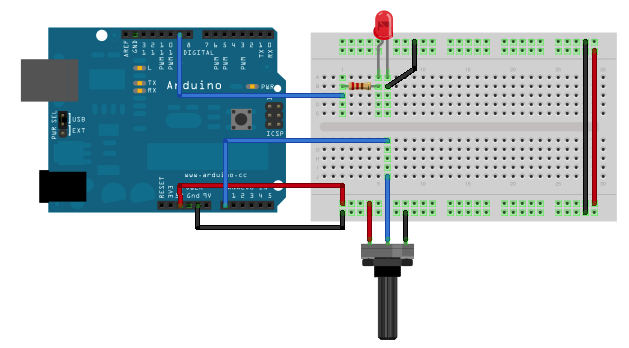
\includegraphics[scale=0.3]{img/analogio/analog_In_lab_pot_and_LED_bb.png}
 \caption{analog In lab pot and LED bb}
 \label{analog In lab pot and LED bb}
\end{figure}


\begin{figure}[!htb]
 \centering
 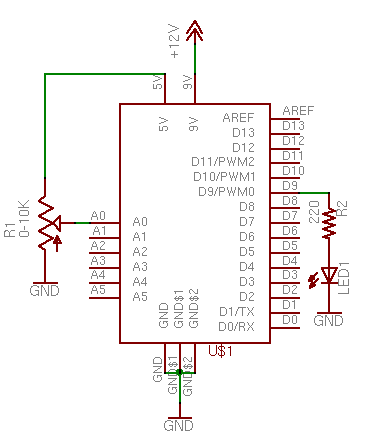
\includegraphics[scale=0.6]{img/analogio/arduino_analog_input_schem.png}
 \caption{arduino analog input schem}
 \label{arduino analog input schem}
\end{figure}

\section{Program the Module}

Program your Arduino with the following code:

\begin{lstlisting}[language=C]
 int potPin = 0;    // Analog input pin that the potentiometer is attached to
 int potValue = 0;   // value read from the pot
 int led = 9;    // PWM pin that the LED is on.  n.b. PWM 0 is on digital pin 9

 void setup() {
   // initialize serial communications at 9600 bps:
   Serial.begin(9600); 
   // declare the led pin as an output:
   pinMode(led, OUTPUT);
 }

 void loop() {
   potValue = analogRead(potPin); // read the pot value
   analogWrite(led, potValue/4);  // PWM the LED with the pot value (divided by 4 to fit in a byte)
   Serial.println(potValue);      // print the pot value back to the debugger pane
   delay(10);                     // wait 10 milliseconds before the next loop
 }
\end{lstlisting}

When you run this code, the LED should dim up and down as you turn the pot, and the value of the pot should show up in the debugger pane.

\section{Other variable resistors}

You can use many different types of variable resistors for analog input. For example, the pink monkey in the photo below has his arms wired with flex sensors. These sensors change their resistance as they are flexed. When the monkey's arms move up and down, the values of the flex sensors change the brightness of two LEDs. The same values could be used to control servo motors, change the frequency on a speaker, or move servo motors.

\begin{figure}[!htb]
 \centering
 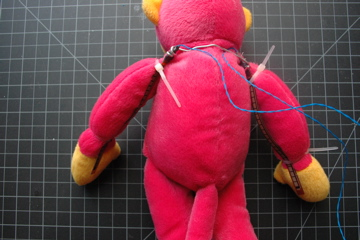
\includegraphics[scale=0.6]{img/analogio/monski_analog.jpg}
 \caption{monski analog}
 \label{monski analog}
\end{figure}

\begin{figure}[!htb]
 \centering
 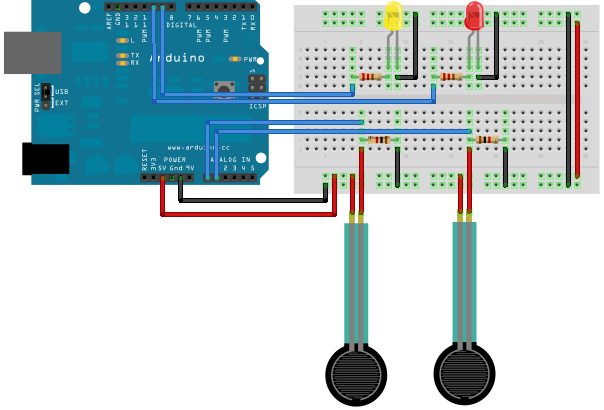
\includegraphics[scale=0.6]{img/analogio/analog_in_lab_monkey_arms_bb.png}
 \caption{analog in lab monkey arms bb}
 \label{analog in lab monkey arms bb}
\end{figure}

\begin{figure}[!htb]
 \centering
 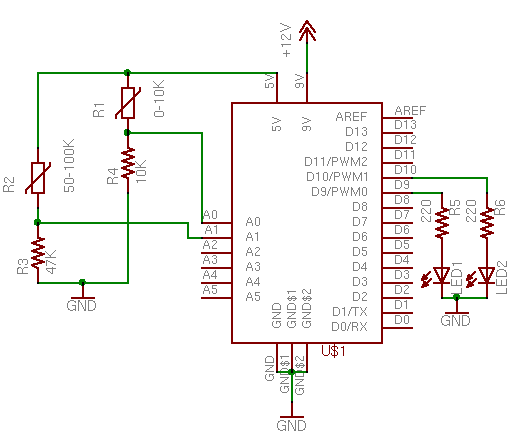
\includegraphics[scale=0.6]{img/analogio/arduino_analog_in2_schem.png}
 \caption{arduino analog in2 schem}
 \label{arduino analog in2 schem}
\end{figure}


The circuit above works for any variable resistor. It's called a voltage divider. There are two voltage dividers, one on analog in 0 and one on analog in 1. The fixed resistor in each circuit should have the same order of magnitude as the variable resistor's range. For example, if you're using a flex sensor with a range of 50 - 100 kilohms, you might use a 47Kohm or a 100Kohm fixed resistor. If you're using a force sensing resistor that goes from inifinity ohms to 10 ohms, but most of its range is between 10Kohms and 10 ohms, you might use a 10Kohm fixed resistor.

The code above assumes you are using a potentiometer, which always gives the full range of analog input, which is 0 to 1023. Dividing by 4 gives you a range of 0 to 255, which is the full output range of the analogWrite() command. The voltage divider circuit, on the other hand, can't give you the full range. The fixed resistor in the circuit limits the range. You'll need to modify the code. First find out your range, open the serial monitor and watch the printout as you wave your hand over the photocell. Note the maximum value and the minimum value. Then you can map the range that the photocell actually gives as input to the range that the LED needs as output. For example, if your photocell gives a range from 400 to 900, you'd do this:


\begin{lstlisting}[language=C]
 // map the sensor vaue from the input range (400 - 900, for example) to the output range (0-255):
 int brightness = map(sensorValue, 400, 900, 0, 255);
 analogWrite(led, brightness);
Here's an alternate version of the program above for this circuit:
 int potPin = 0;    // Analog input pin that the potentiometer is attached to
 int sensorValue = 0;   // value read from the analog sensor
 int led = 9;    // PWM pin that the LED is on.  n.b. PWM 0 is on digital pin 9

 void setup() {
   // initialize serial communications at 9600 bps:
   Serial.begin(9600); 
   // declare the led pin as an output:
   pinMode(led, OUTPUT);
 }

 void loop() {
   sensorValue = analogRead(potPin); // read the pot value

   // map the sensor vaue from the input range (400 - 900, for example) 
   // to the output range (0-255). Change the values 400 and 900 below
   // to match the range your analog input gives:
   int brightness = map(sensorValue, 400, 900, 0, 255); 

   analogWrite(led, brightness);  // set the LED brightness with the result
   Serial.println(sensorValue);   // print the pot value back to the debugger pane
   delay(10);                     // wait 10 milliseconds before the next loop
 }
\end{lstlisting}

\section{Get creative}

This is a suggestion for the Stupid Pet Trick assignment. You can do any project you wish as long as it demonstrates your mastery of the lab exercises and good physical interaction. This is just one suggestion.
Make a luv-o-meter with analog inputs. A luv-o-meter is a device that measures a person's potential to be a lover, and displays it on a graph of lights. In gaming arcades, the luv-o-meter is usually a handle that a person grips, and his or her grip is measured either for its strength or its sweatiness. But your luv-o-meter can measure any analog physical quantity that you want, providing you have a sensor for it. Make sure the display is clear, so the participant knows what it means, and make sure it is responsive.

